We now turn to the experiment of recording the spectra of the fluctuating membrane, which later on can be calibrated. From the calibrated spectrum we can extract the effective mechanical mode temperature by integrating the mechanical resonance as shown in section \ref{sec:xrms}. We record the spectra from the AC output from the detector, which is \SI{5}{\mega\hertz} low-pass\footnote{Mini-Circuit NLP-5+} filtered twice to avoid aliasing, before sending the signal to a data acquisition-card\footnote{Adlink PCI-9846H}. To generate a calibration tone the EOM is driven by a signal generator\footnote{Rohde \& Schwartz SMC110A} at a frequency of \SI{2.185}{\mega\hertz} and a power of \SI{-56}{\deci\bel\milli}. The spectra is recorded averaging 50 times with a sample rate of \SI{10}{\mega} and a resolution bandwidth of \SI{10}{\hertz} for each detuning, after the OMIT trace while maintaining the lock.

The calibration of the spectra is done according to the routine sketched in \cite{gorodetsky2010}. We calibrate the spectra using the scaling factor

\begin{equation}
F_{calib} = \frac{\beta^2f_{mod}^2}{A_{calib}}\left(\frac{x_{zpf}}{g_0}\right)^2,
\end{equation}
\noindent
where $f_{mod}$ is EOM modulation frequency, $A_{calib}$ is the area under the calibration tone and $\beta$ is magnitude of phase modulation in the light ($\beta = \sqrt{P_{eom}R(\pi/V_{\pi})^2}$) as in \cite{black2001}. Our $V_{\pi}$ is measured to be \SI{2.09}{\volt}. We use the $g_0$ found from the OMIT fit seen in figure \ref{fig:omit_fit_g0}. The new spectra we get from the calibration procedure around the mechanical resonance are shown in figure \ref{fig:spec_calib} for a selection of relevant detunings.

\begin{figure}[H]
\centering
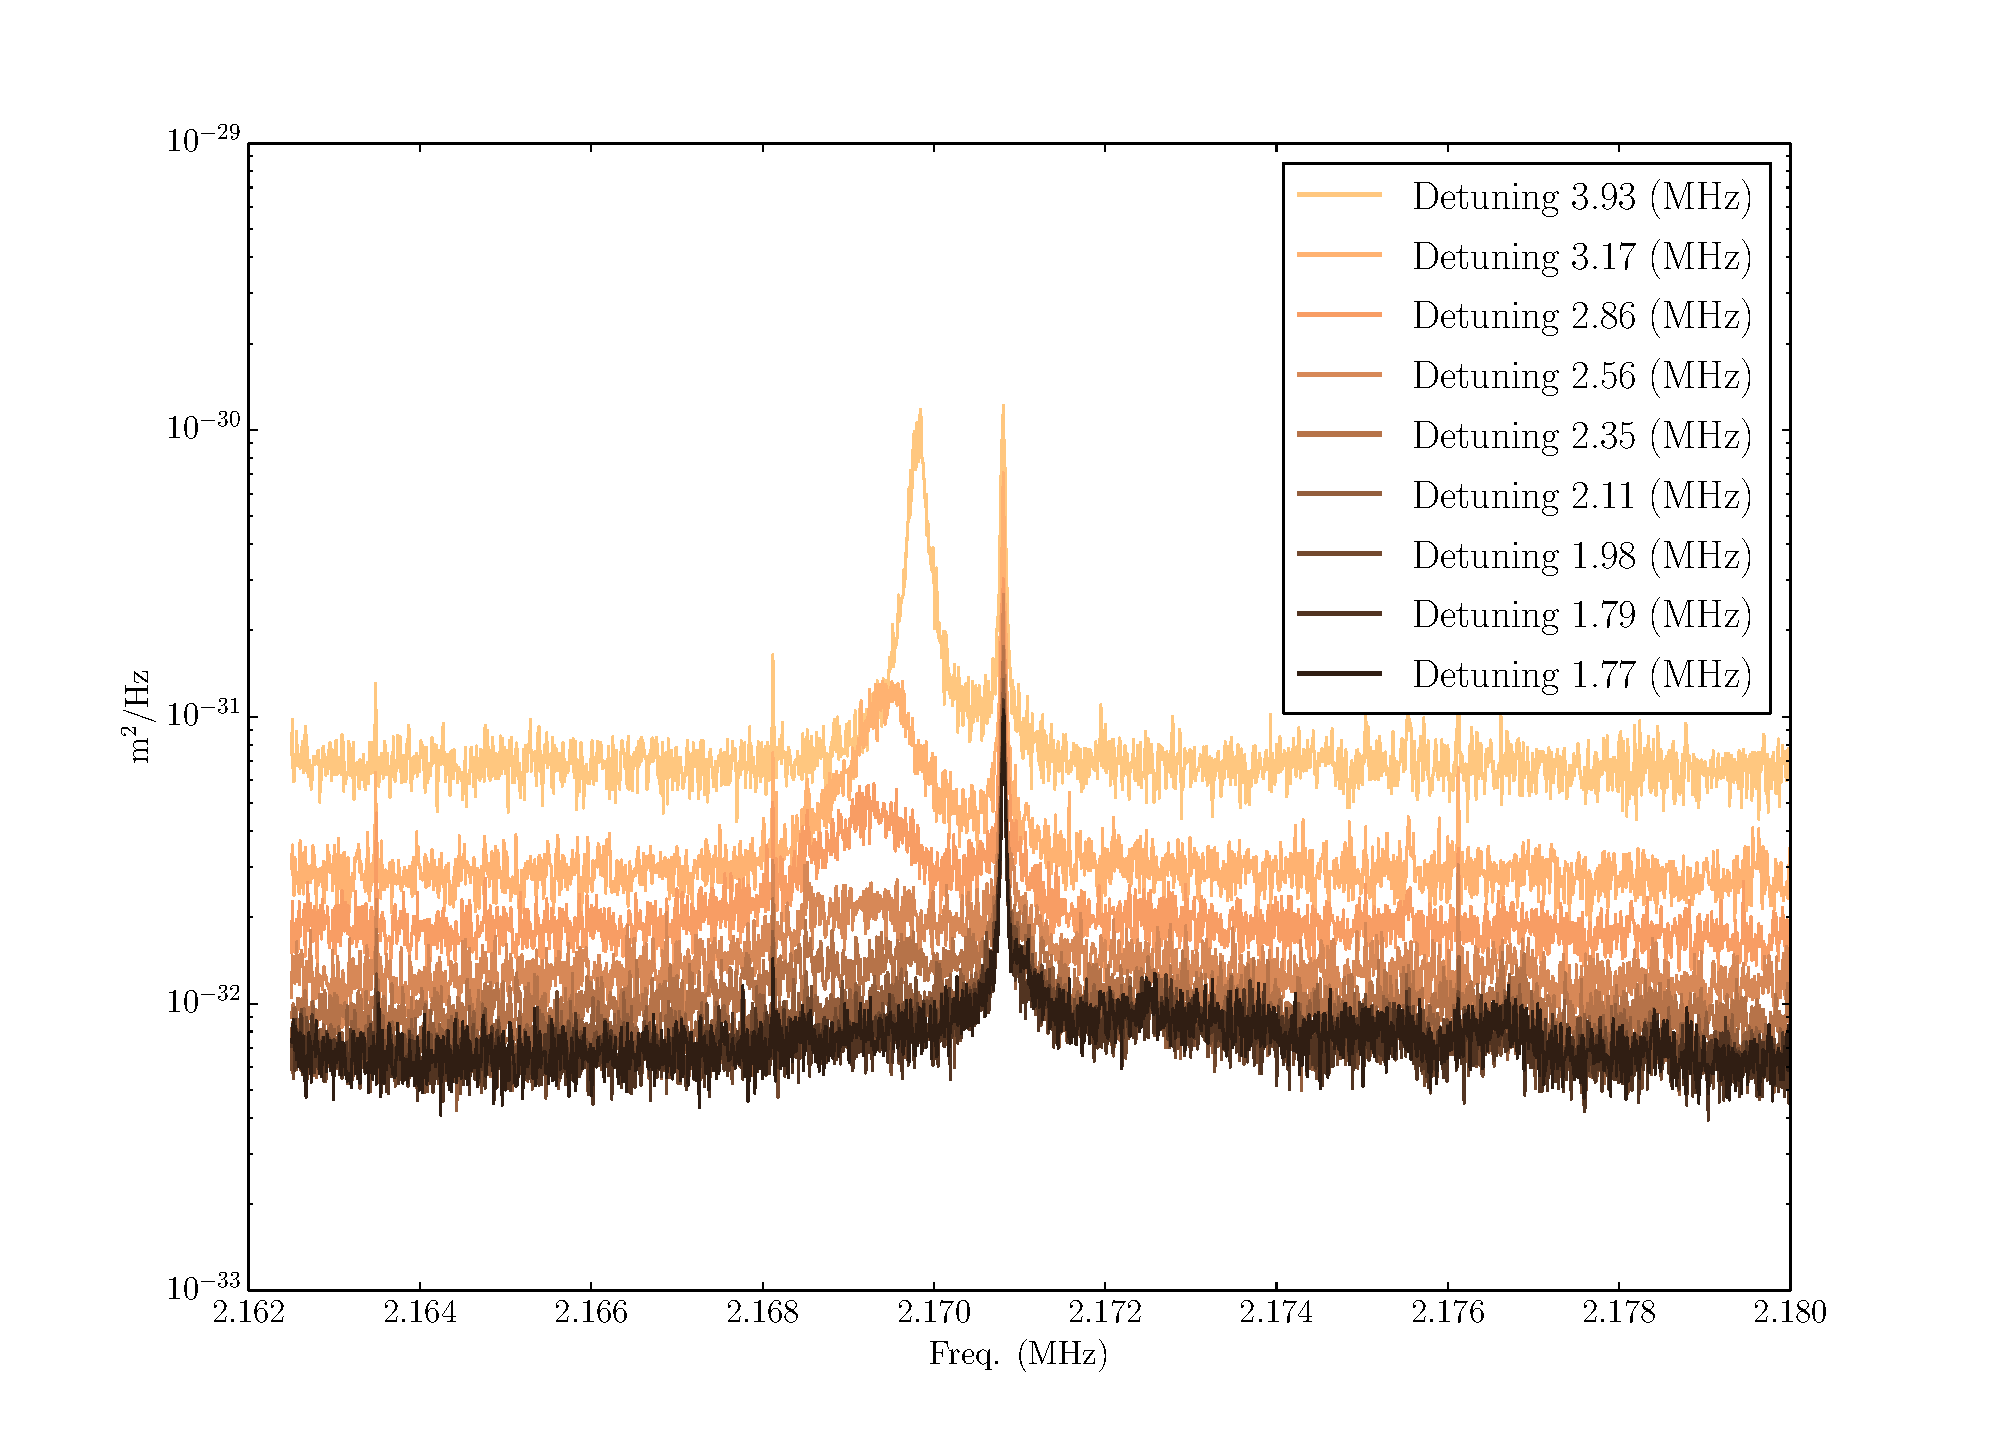
\includegraphics[scale=0.45]{analysis/cal_spec_newest0.pdf}
\caption{Broadening of the mechanical resonance in calibrated spectra as the detuning is changed towards optimal condition for cooling. The large peak at \SI{2.171}{\mega\hertz} is unfortunately unwanted noise.}
\label{fig:spec_calib}
\end{figure}

We see in the figure above that the mechanical peak gets broadened as expected from theory as we detune towards the optimal condition for sideband cooling. The mechanical resonance gets hard to distinguish form noise, but nevertheless the signal-to-noise ratio never drops below unity for the full detuning series. We are quite unlucky because a noise peak, which was not present in preliminary test, is showing right on top of the broadened resonance. The noise is unfortunate, but we can work around it, when fitting a Lorentzian to mechanical peak for finding the effective damping, by either fitting a double-Lorentzian to the noise and mechanical peak or simply by cutting out the unwanted noise, since it is static as seen in figure \ref{fig:spec_calib}. We did both and they yielded roughly the same result, but the latter was more invariant/robust to changes like fitting range, i.e. the number of points fitted. A plot showing the fitted effective damping from the spectra compared to the effective damping obtained from the OMIT fit can be seen in figure \ref{fig:spec_eff_damp}.

\begin{figure}[H]
\centering
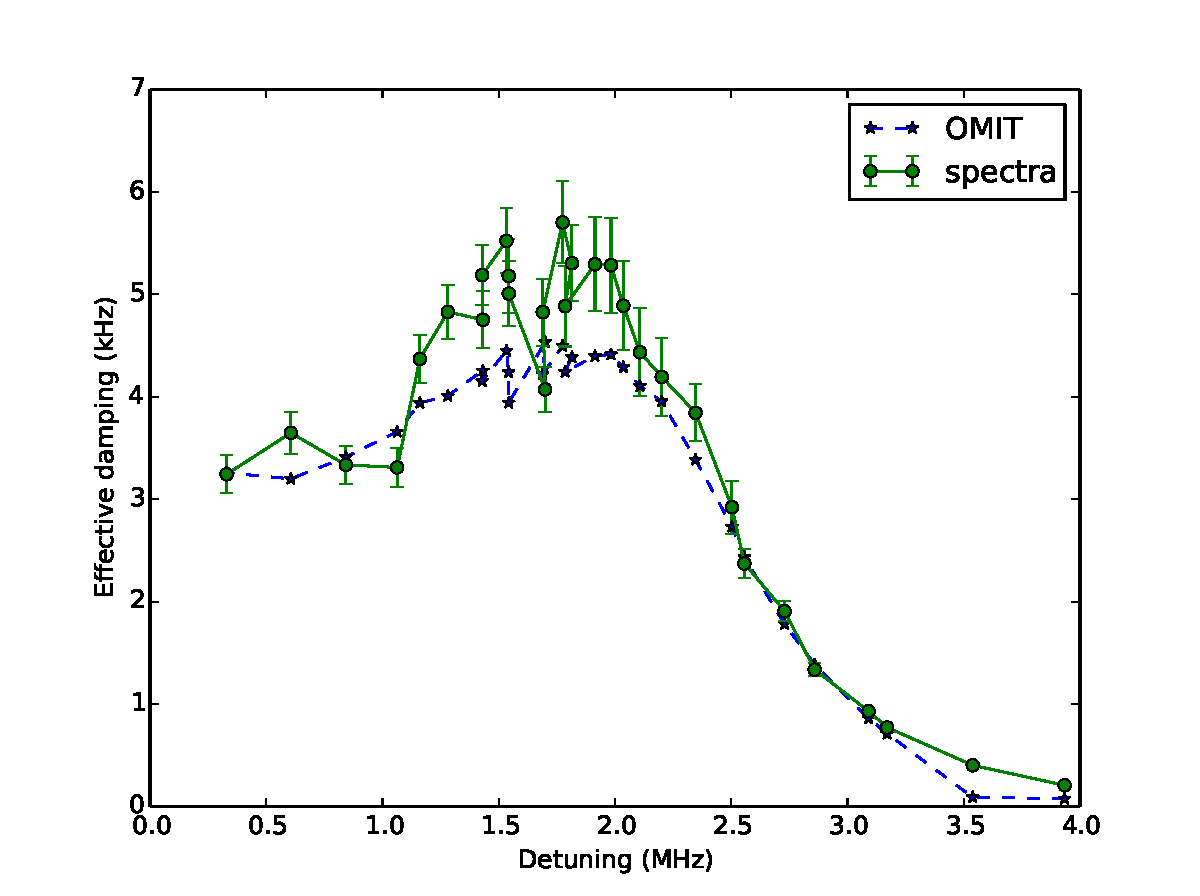
\includegraphics[scale=0.7]{analysis/eff_damp_newest.pdf}
\caption{Effective damping from the Lorentzian fit of the mechanical resonance compared with the prediction made from the OMIT fit.}
\label{fig:spec_eff_damp}
\end{figure}

The OMIT fit seems to consistently underestimate the effective broadening of the mechanical mode, for detunings near the mechanical resonance, but they follow the same tendency and the agreement between model and data is good. From the amplitude of the Lorentzian fit we get the calibrated area beneath the mechanical mode. The area determines the effective temperature of mechanical mode by \eqref{eq:t_eff}. Using the effective temperatures and Bose-Einstein distribution, we calculate the mean phonon occupancy $\bar{n}_{phonon} = \left[e^{\hbar\Omega_m/k_BT_{eff}} - 1\right]^{-1}$. We shown the mean phonon occupation number as function of detuning in figure \ref{fig:phonon_occ}.

\begin{figure}[H]
\centering
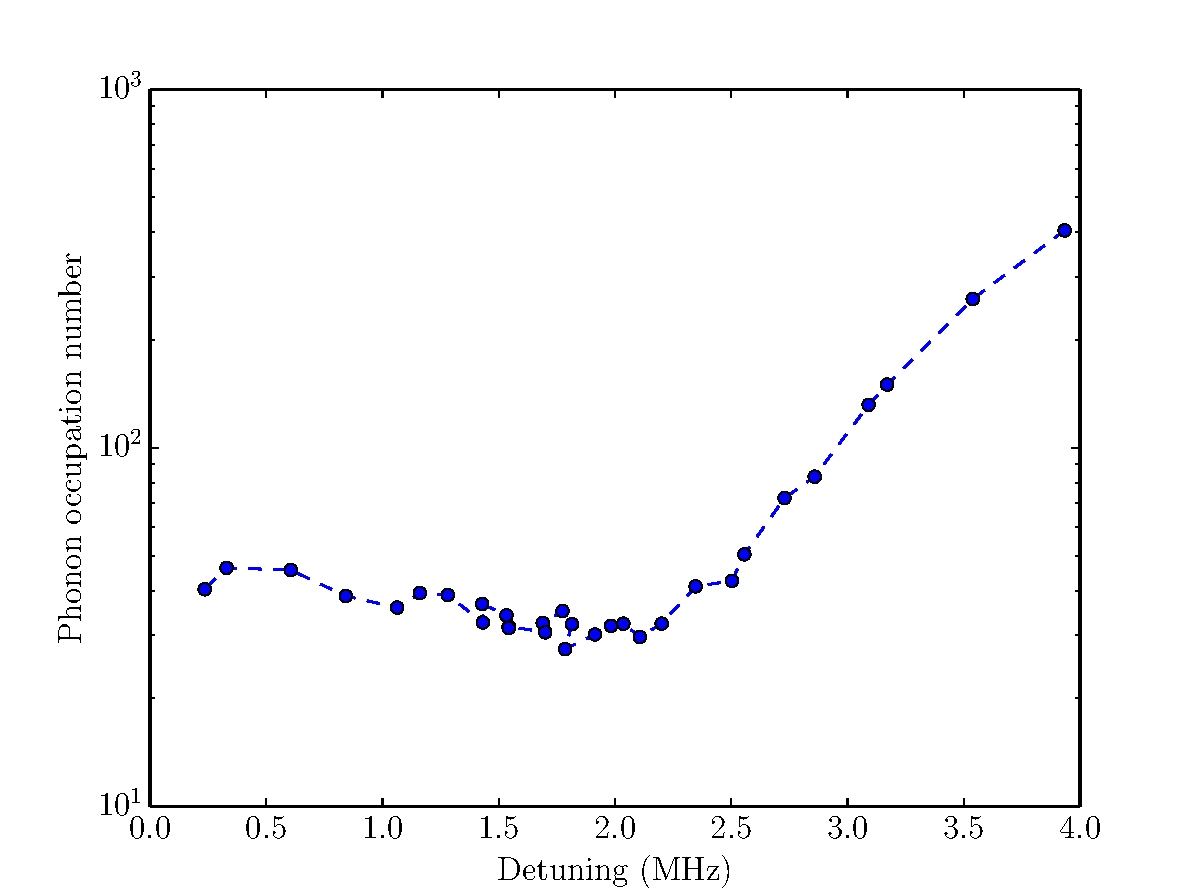
\includegraphics[scale=0.7]{analysis/phono_occ.pdf}
\caption{The extrapolated mean phonon occupancy of the mechanical (3,3)-mode.}
\label{fig:phonon_occ}
\end{figure}

The minimum mean phonon occupancy from the recorded spectra is $\bar{n}_{phonon}^{min} \approx 27\substack{+11 \\ -7}$. The errors is a combination of the easy accessible errors from the fitted $g_0$ and the error on the fitted area. We have not included more complex uncertainties, due to time constrains, from $V_{\pi}$, the calculated cavity photon number $\bar{n}_{cav}$ and corrections from the transduction function of the signal sent to the EOM.